\pagebreak
\subsection{Electrical Design}

\subsubsection{Block Diagram}
\label{sec:4.5.1}

The electronics design can be seen in Figure \ref{fig:electronics-block-diagram} which shows the connections, grounding, voltages, and signals. 

\begin{figure}[H]
    \begin{align*}
        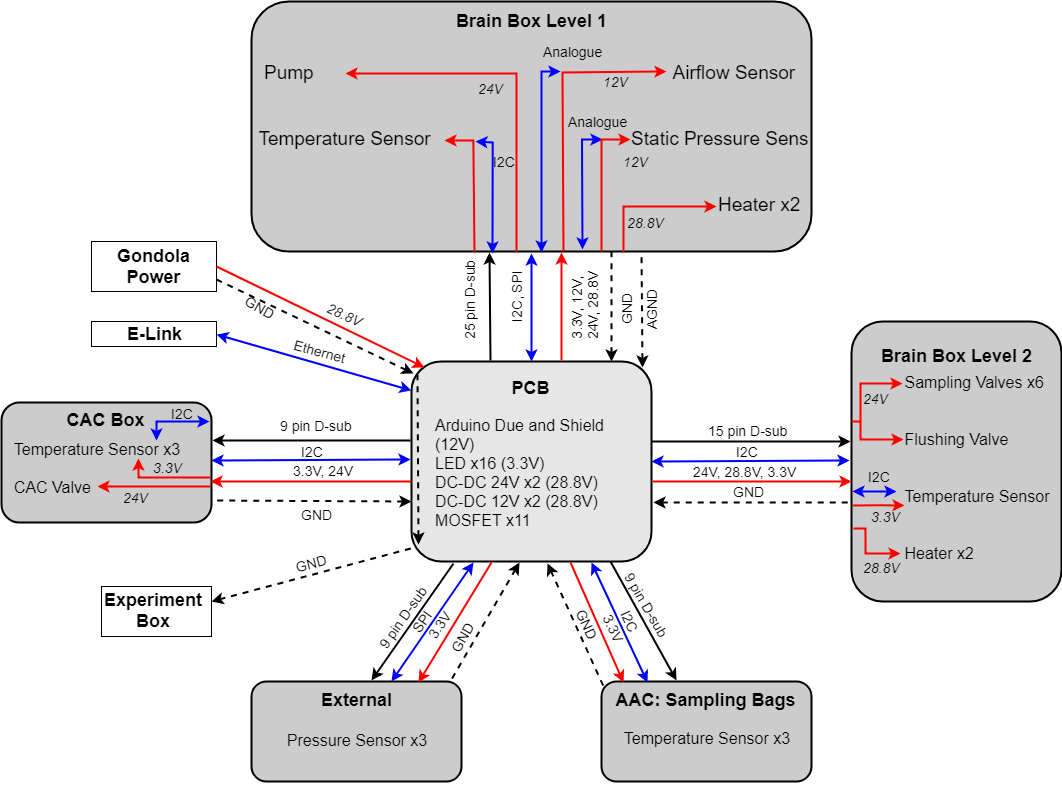
\includegraphics[width=16cm]{4-experiment-design/img/Electrical_Block_diagram.png}
    \end{align*}
    \caption{Block Diagram for all Electronic Components Showing the Connection, Signal and Power Connections.}\label{fig:electronics-block-diagram}
\end{figure}

Most of the electronics were located in the Brain inside the AAC box. However, there were six distinct areas:

\begin{enumerate}
    \item The Brain level 3, where the PCB is located with the Arudino and shield, two 24 V DC-DC, two 12 V DC-DC, 11 MOSFETs and 16 LEDs.
    \item The Brain level 2, where the valve manifolds with six sampling valves, the flushing valve, two heaters, airflow sensor, static pressure sensor and one temperature sensor were located.
    \item The Brain level 1, where the pump, two heaters and one temperature sensor were located.
    \item The AAC box, where 3 ambient temperature sensors were located.
    \item The CAC box, where the CAC valve and 3 ambient temperature sensors were located.
    \item Outside of the experiment box, where 3 ambient pressure sensors were located.
\end{enumerate}

From the PCB, on level 3, five D-sub connectors were used to connect to the other five areas. Fifteen pin connectors were used for level 1 and level 2. For the CAC box, AAC box sampling bags area, and the external pressure sensors, nine pin connectors were used. In addition there was a connection to the gondola power and gondola E-link.

All of the power distribution was done through the PCB using two 24 V DC-DC and two 12 V DC-DC converters in parallel with a forwarding diode.  
\begin{itemize}
  \item $28.8 \, V \Longrightarrow 24 \, V $ By DC-DC converters
  \item $28.8 \, V \Longrightarrow 12 \, V$ By DC-DC converters
  \end{itemize}
The heaters did not require the voltage to be stepped down and so were powered directly from the gondola battery.

The Arduino was used to control all of the sensors, valves, heaters and the pump from the PCB. Sensors were directly connected to the Arduino. The valves, heaters and the pump were connected via a switching circuit.

The LEDs were used as visual indicators that displayed whether different parts of the circuit are active or not. They gave indications on the status of the valves, pump, heaters, DC-DC converters and Arduino. 

Grounding was done following a distributed single point grounding, with all ground connections meeting at a single star point ensuring there were no floating grounds. As not all components were connected via DC-DC converters the experiment was not isolated from the gondola power supply therefore there was a connection between the star point and the gondola ground. The star point was located on the main PCB board which was then grounded to the experiment box. The grounding can be seen in Figure \ref{fig:electronics-block-diagram} where it is indicated by dashed lines labeled GND. The analog sensors that were used on level 1 in the brain used a separate grounding wire(AGND) onto the main PCB where there was a separate trace connecting to the ground pins on the Arduino board. Furthermore  the  upper  and  lower  level  of  the  main PCB board were making use of the common grounding plane where possible.

\subsubsection{Miniature Diaphragm Air Pump}
The pump which was selected was the 850.1.2. KNDC B, Figure \ref{fig:pumppic}, which is manufactured by KNF. One of the reasons this pump was selected is that it was successfully flown on a similar flight in the past where it managed to pump enough air at 25 km altitude to have 180 mL remaining at sea level \cite{LISA}. However, to ensure the pump will operate as intended, several tests were carried out. These tests --- 4, 5, 18, 28 and 29, can be seen in Tables \ref{tab:vacuum-test}, \ref{tab:thermal-test}, \ref{tab:pump-low-pressure-test}, \ref{tab:pump-operation-test}, and \ref{tab:pump-current-pressure-test}.

At sea level conditions the pump was tested and found to have a flow rate of 8.0 L/min and a current draw of 250 mA. The peak current draw was recorded as 600 mA which lasts for less than one second and occurs when the pump is switched on. 

From the results of Test 18, in Section \ref{sec:ExpecterResults}, the flow rate was shown to be around 3.36 L/min at the lowest pressure that will be seen in flight. This was in line with requirement D23. The results found in Test 28, in Section \ref{sec:test28result}, appeared to be inline with the information given by the manufacturer, seen in Figure \ref{fig:pumpflowcur}.  The highest continuous current draw expected from the pump was 185 mA when the experiment is at 12 km altitude and was expected to decrease as we increase in altitude. While it appeared that the pump increased in current draw at around 6 km there was no plan to sample below 12 km therefore the highest current draw was taken from 12 km. As the pump had a peak current of 600 mA when it switches on, the mosfet and DC-DC power have been chosen to be able to withstand this demand. 

\begin{figure}[H]
    \begin{align*}
        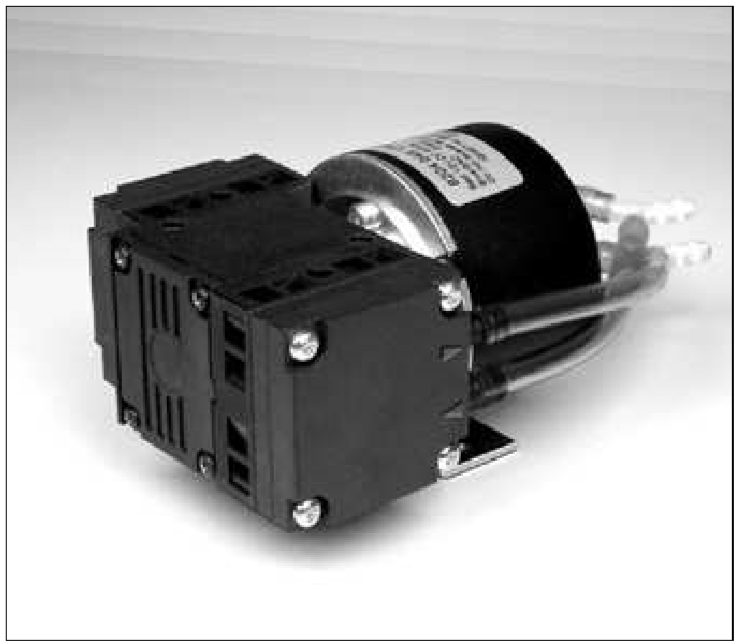
\includegraphics[width=6cm]{4-experiment-design/img/pump-850-1-2-kndc-b.png}
    \end{align*}
    \caption{KNF 850.1.2. KNDC B Miniature Diaphragm Pump.}\label{fig:pumppic}
\end{figure}


\begin{figure}[H]
    \begin{align*}
        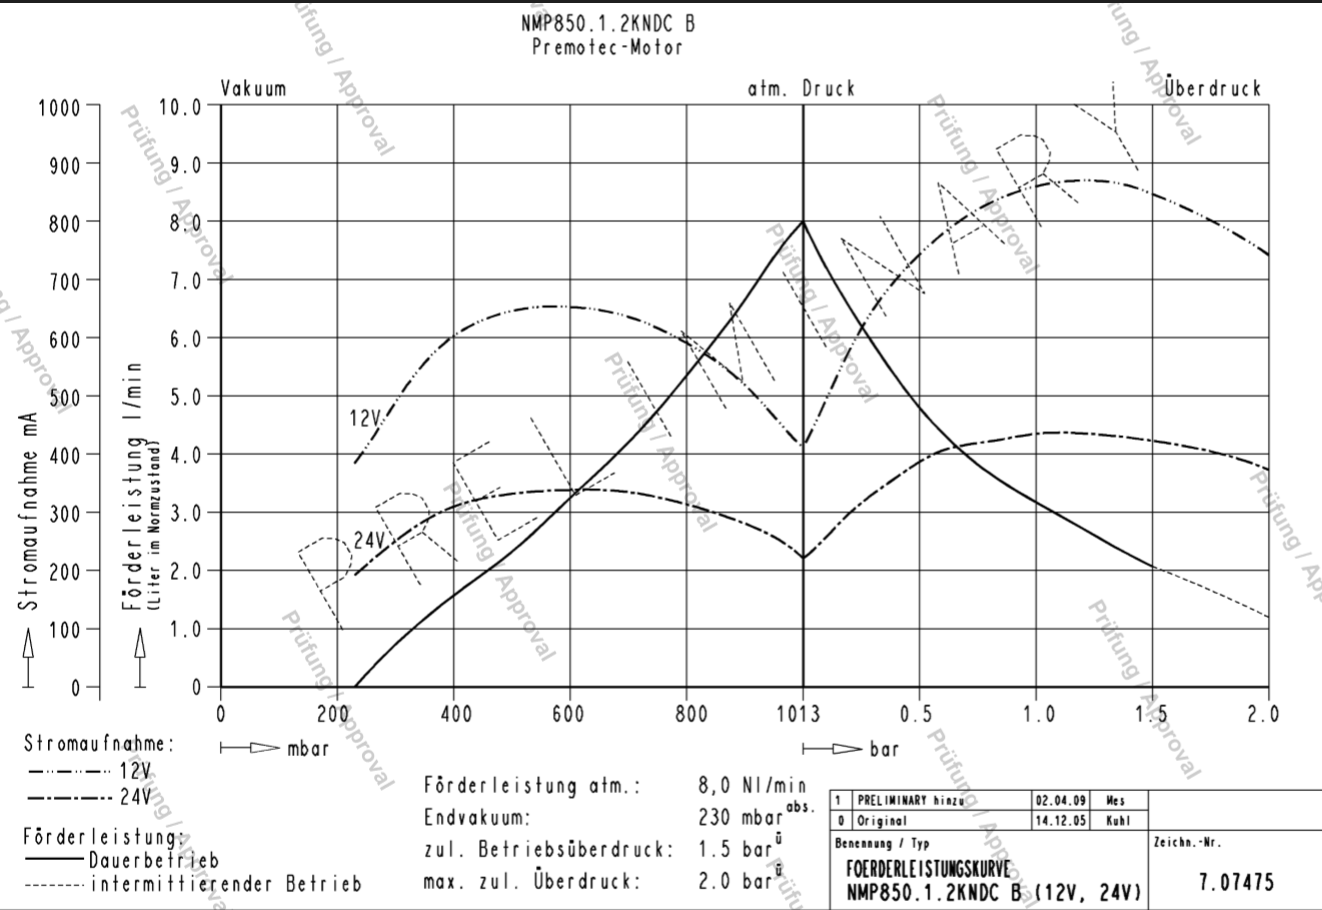
\includegraphics[width=15cm]{4-experiment-design/img/pump-flow-rate-current-graph.png}
    \end{align*}
    \caption{KNF 850.1.2. KNDC B Flow Rate and Current Draw to Pressure Graph.}\label{fig:pumpflowcur}
\end{figure}


\subsubsection{Electromagnetically Controlled Valves}
Filling the sampling bags was controlled by solenoid valves. The solenoid valves selected were model VDW23-5G-1-H-Q, seen in Figure \ref{fig:valve}, manufactured by SMC. These valves were normally closed through out the experiment with zero power consumption and opened, when given power, to fill up the sampling bags at specific altitudes. In addition one valve was on the CAC, in order to seal the coil at the end of the flight and another at the end of the AAC tubing, flushing valve, in order to flush the system.  The valves selected for these are model VDW22UANXB, Figure \ref{fig:valve}. The CAC valve was opened shortly after take off and remained open the whole flight. This valve was closed shortly before landing. The flushing valve was opened before sampling in order to ensure the air in the tubes was from the correct altitude.

\begin{figure}[H]
    \begin{align*}
        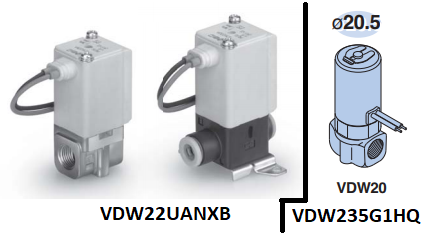
\includegraphics[width=6cm]{4-experiment-design/img/valves.png}
    \end{align*}
    \caption{SMC Solenoid Valves, VDW22UANXB on the Left, VDW23-5G-1-H-Q on the Right.}
    \label{fig:valve}
\end{figure}

The port size of the valves was 1/8" which is compatible with the gas analyzer. The coil inside can withstand temperatures from -20 to 110 $\degree{C}$ which was suitable for flight operations at high altitudes. These valves can operate under a maximum pressure drop of 133 Pa. Valves from the same series were flown before to the stratosphere and provided successful results \cite{LISA} however, the valves were tested at low temperature and pressure to check they still operate as intended. The test results can be seen in Test 4, Table \ref{tab:vacuum-test} and Test 5, Table \ref{tab:thermal-test}.
 
\subsubsection{Switching Circuits}
The valves, pump and heaters were not powered by the Arduino but they were still controlled by it. In order to allow this control a connection was made for each component to the Arduino with a switching circuit. This switching circuit used eleven MOSFETs, model IRLB8748PBF, Figure \ref{fig:mosfet}, to control which components were turned on at which time.

\begin{figure}[H]
    \begin{align*}
        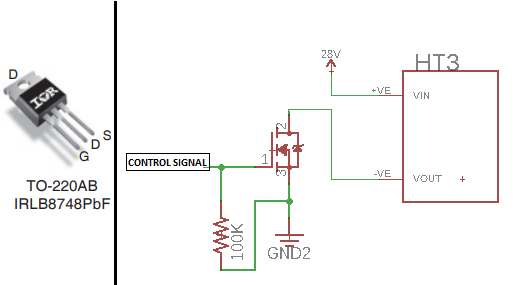
\includegraphics[width=10cm]{4-experiment-design/img/mosfet.png}
    \end{align*}
    \caption{Figure Showing an Image of the 30V,78A,75W MOSFET, Model Number IRLB8748PBF on the Left and the Schematic for the Switching Circuit for One Heater on the Right.}\label{fig:mosfet}
\end{figure}

\subsubsection{Schematic}

The schematics show all the components and how they are connected, the full schematics can be seen in Figure \ref{fig:Schematic}. There are four requirements for the the power distribution given below:

\begin{itemize}

    \item $28.8 \, V$ for the heaters.  
    
    \item $28.8 \, V \Longrightarrow 24 \, V$ for the pump and valves.
    
    \item $28.8 \, V \Longrightarrow 12 \, V$ for the airflow sensor, static pressure sensor and Arduino due.
    
    \item $3.3 \, V$ for the temperature and pressure sensors. 
    
\end{itemize}

The voltage available from gondola power is 28.8 V, therefore the heaters were connected directly to the main power supply. For the rest of the components, two 24 V and two 12 V DC-DCs in parallel were used to make sure if one of them fails then the other can take over. The circuitry can be seen in Figure \ref{fig:dc-dc-redun}. All the valves and the pump were then powered through the 24 V DC-DCs. To step down the voltage from 28.8 V to 12 V to power the airflow sensor, static pressure sensor and the Arduino, two 12 V DC-DCs in parallel were used for redundancy purposes. Finally, to power the temperature and external pressure sensors, 3.3 V is required which is supplied by the Arduino board. 

To meet the requirements of the pneumatic subsystem, a static pressure sensor was chosen to measure the pressure inside the tubes and bags. This analogue pressure sensor operated on 12 V so could share the same power line as the airflow sensor and Arduino.


\begin{figure}[H]
    \begin{align*}
        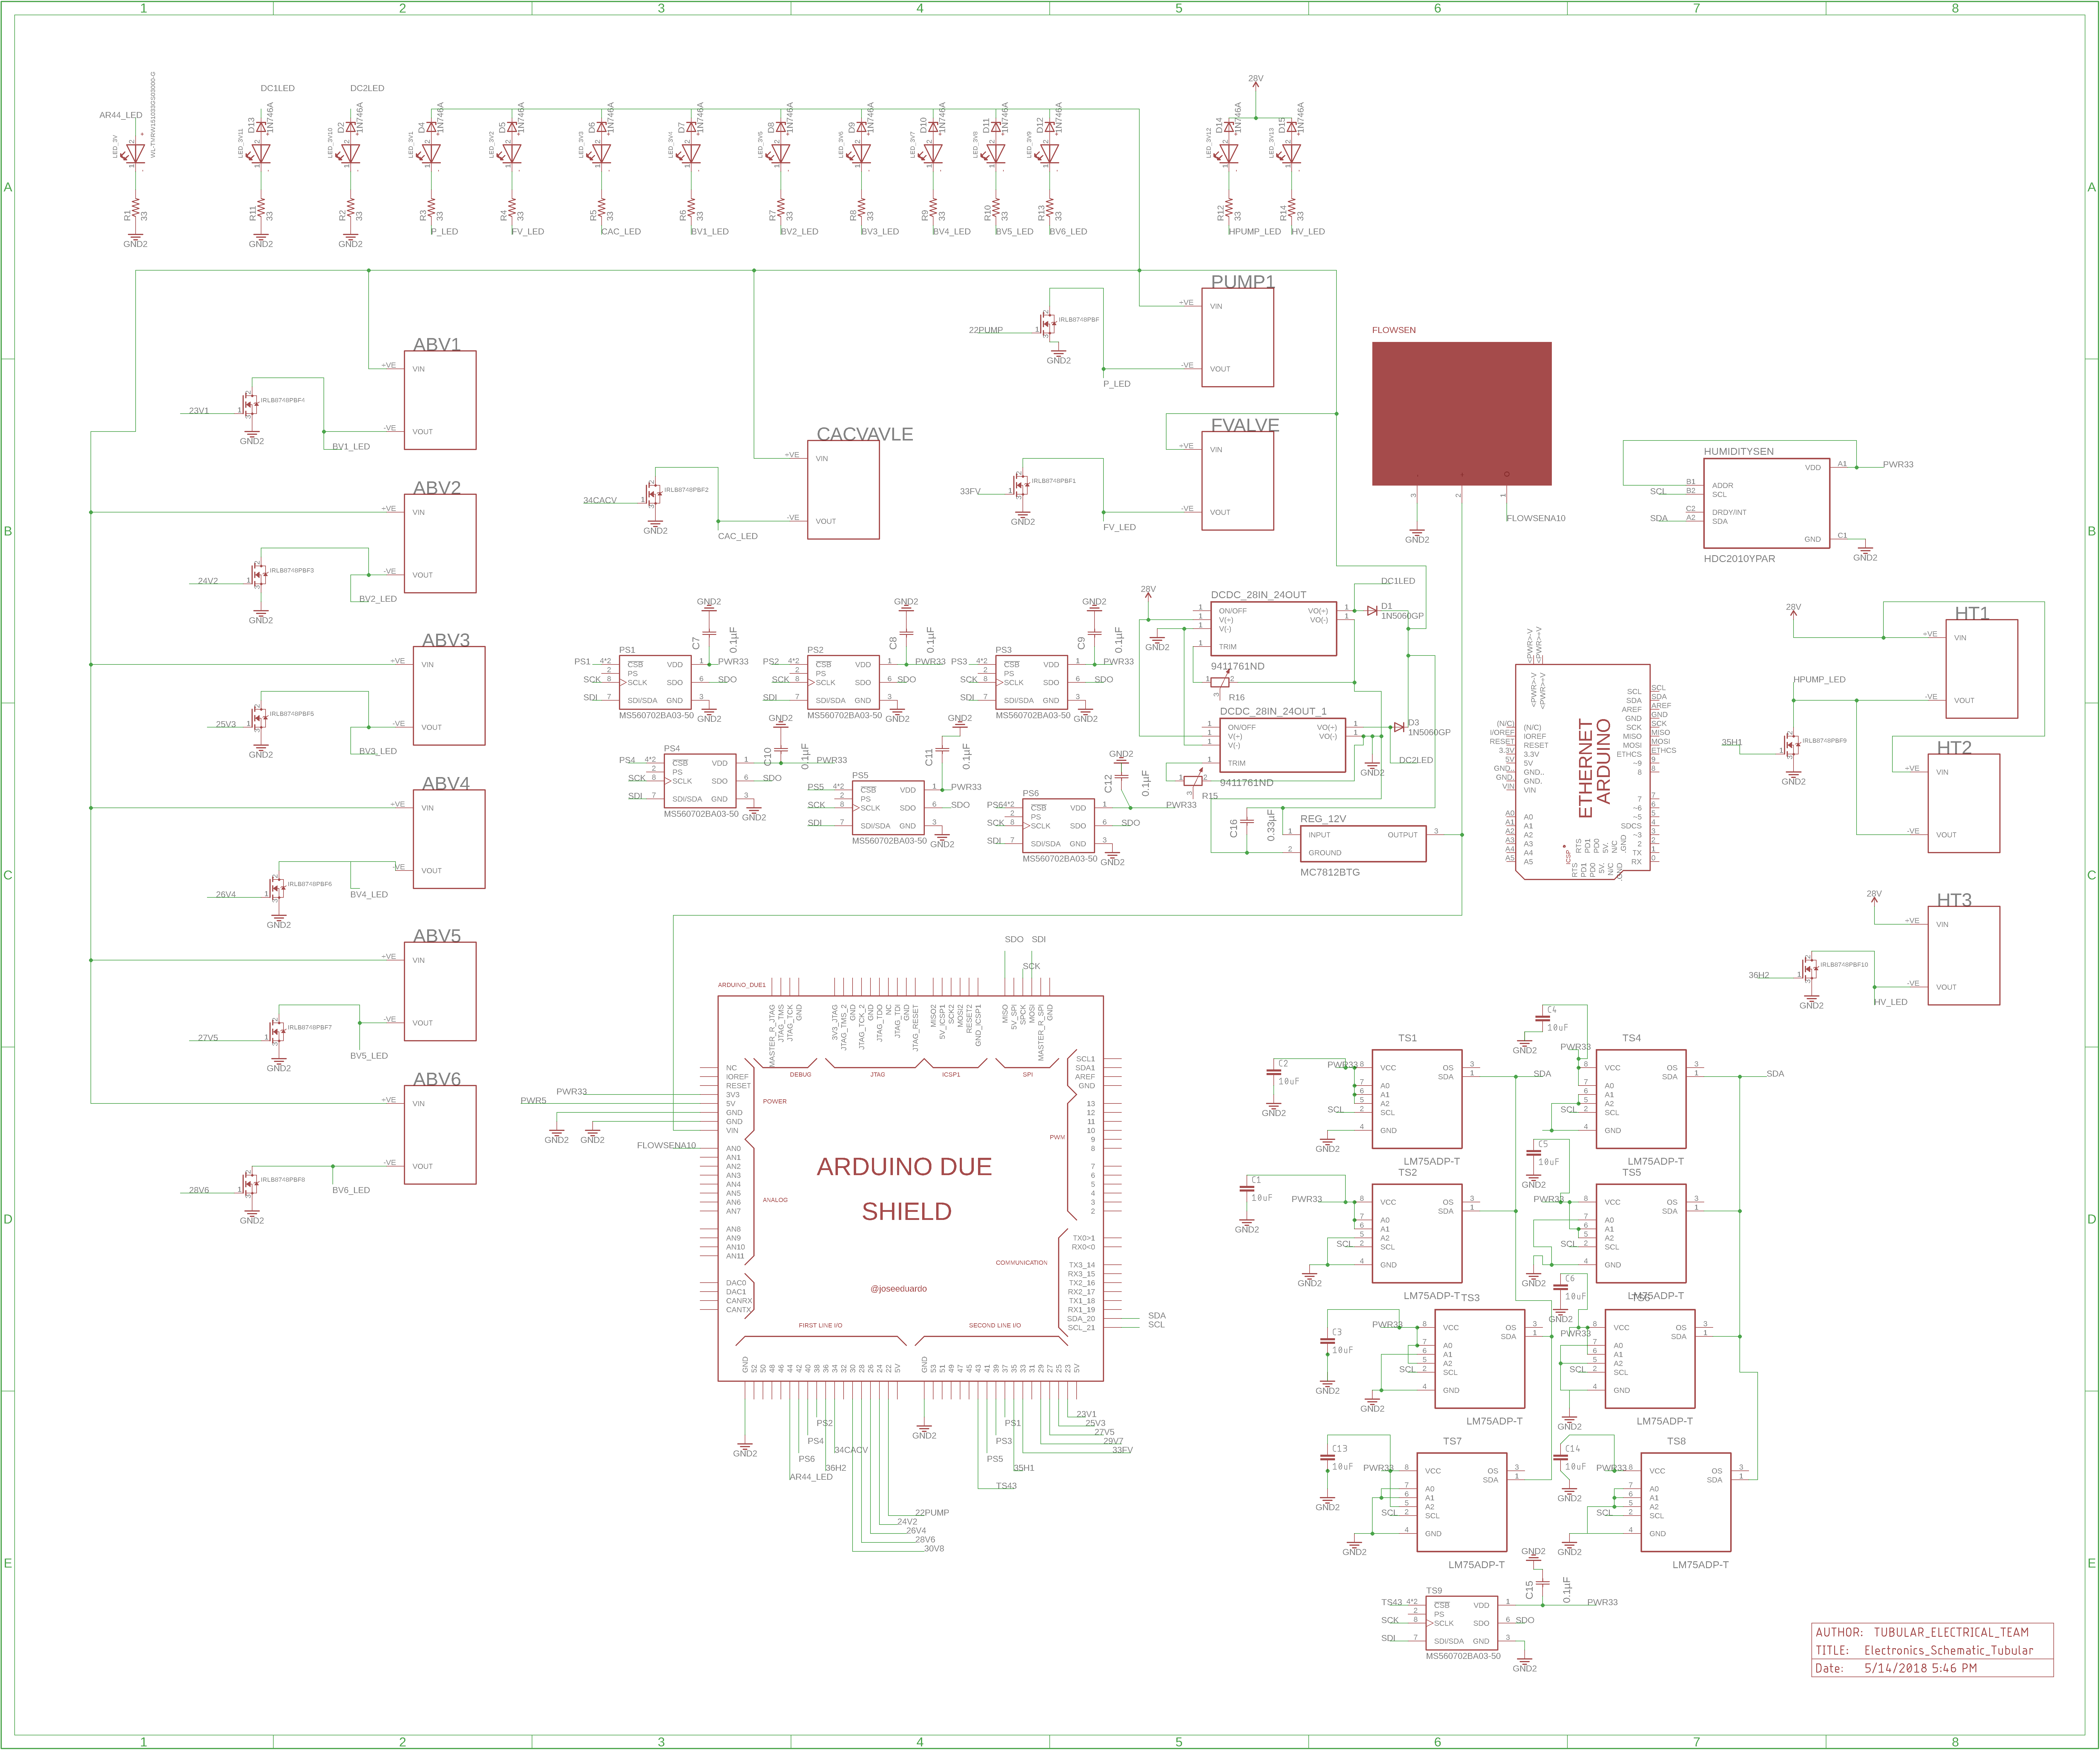
\includegraphics[width=16cm]{4-experiment-design/img/Schematics.png}
    \end{align*}
    \caption{Schematic for All of the Electronics on Board TUBULAR. This can also be Found at https://rexusbexus.github.io/tubular/img/electrical-design-schematics.png}\label{fig:Schematic}
\end{figure}

\begin{figure}[H]
    \begin{align*}
        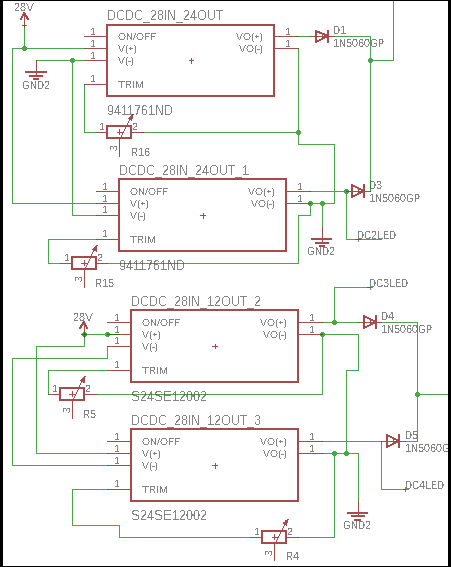
\includegraphics[width=13cm]{4-experiment-design/img/DCDC-converter-redundancy.png}
    \end{align*}
    \caption{Schematic Showing the DC-DC Redundancy of Both 24 V  and the 12 V DC-DC Converters.}\label{fig:dc-dc-redun}
\end{figure}


\subsubsection{PCB Layout}

All electronic control circuits were gathered on a single PCB on level 3 of the Brain. The PCB contained the Arduino due, switching circuits, indication LEDs, a temperature sensor, the power system and all necessary connectors. The connectors were divided so that each connector's wires goes to the same level of the Brain to improve cable management. Due to the relocation of components there are some components on level 2, Static pressure sensor and the airflow sensor, which were connected to the level 1 connector. Although this did not produce major problems since both those components have separate connectors on the cable going down to level 1 and does not share any connections with any components on level 1. Thus you could still unplug each level separately since the wires to these two components could just be broken of from the cable loom at the appropriate point. To further improve cable management the shared pins for I2C and SPI were connected to a single pin on each respective D-SUB connector and split up on the respective level. The PCB's components layout can be seen in Figure \ref{fig:PCB-Components-Layout}

\begin{figure}
    \centering
    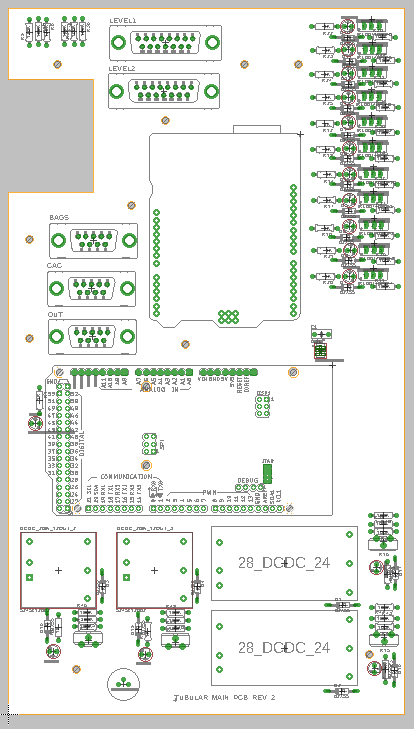
\includegraphics[width=0.7\textwidth]{4-experiment-design/img/PCBLayout.png}
    \caption{PCB Components Layout}
    \label{fig:PCB-Components-Layout}
\end{figure}


The PCB was made using Eagle software and fully sponsored by the Eurocircuits for manufacturing. The traces had a width designed to fit the IPC-2221 standards\cite{IPC-2221B} with extra width added. The PCB layout with traces can be seen in in Appendix \ref{sec:pcbSchematics}. On the main PCB the traces were 1.4mm wide for the nets containing components that consumes higher amounts of current and the ones with lower current requirements had a trace width of 0.3mm. On the pressure sensor PCB all traces were 0.5mm wide.




\raggedbottom